
%(BEGIN_QUESTION)
% Copyright 2008, Tony R. Kuphaldt, released under the Creative Commons Attribution License (v 1.0)
% This means you may do almost anything with this work of mine, so long as you give me proper credit

Qualitatively sketch the {\it derivative} of the function shown here.  In other words, draw another function that describes how {\it quickly} the given curve changes:

$$\includegraphics[width=15.5cm]{i01532x01.eps}$$

\underbar{file i01532}
%(END_QUESTION)





%(BEGIN_ANSWER)

$$\includegraphics[width=15.5cm]{i01532x02.eps}$$

In this particular example:

$$y = f(x) = x^2$$ 

$${dy \over dx} = f'(x) = 2x$$

%(END_ANSWER)





%(BEGIN_NOTES)


%INDEX% Mathematics, calculus: derivative (defined in a graphical sense)

%(END_NOTES)


